\section{Determining Derivative Gain}

Derivative gain is used to decelerate the arm and is activated when the threshold, described in section \ref{sec:thresholds}, is met.
In order for immediate deceleration to occur, derivative gain is bounded to meet the requirement the PD controller be over-damped. 
As with proportional gain, once this requirement is met the exact value for derivative gain is relatively unimportant and should only every have a significant impact on the system if the switching threshold (section \ref{sec:thresholds}) is incorrect.
For robustness, an incorrect switching threshold was assumed when tuning derivative gain.
Figure \ref{fig:kd} shows two system responses where derivative gain is incorrect and increases the time needed to drop the puck. 
Once again, the overshoot is not due to the gains of the PD controller but due to an incorrect controller switching threshold.

%FIXME. 
%When the threshold is reached, the Proportional gain is switched to PD controller. 
%As the figure shows, when the PD controller is very large, it causes the response to be over damped in order to slow the system response as quick as possible. 
%When PD controller is too low, it causes the system response to oscillate before it reaches setting position. 
%Therefore, the over damped drastically increases the settling time for small errors in switching threshold. 

The Simulink block diagram used to implement derivative control may be seen in Figure \ref{fig:simulinkkd}.
Of particular interest is the \q{desensitize} block.
This dead-zone is used to reject small, unstable derivative signals caused by the discreet nature of the encoder. 
Without this block, the system was seen to vibrate excessively at its steady state.
A dead-zone range of $\pm0.07$ was found to effectively eliminate most vibrations.

%Use dead zone to reject small derivative signals.
%Needed as encoder is discreet and small derivative cause vibrations.

\begin{figure}[htp]
    \centering
    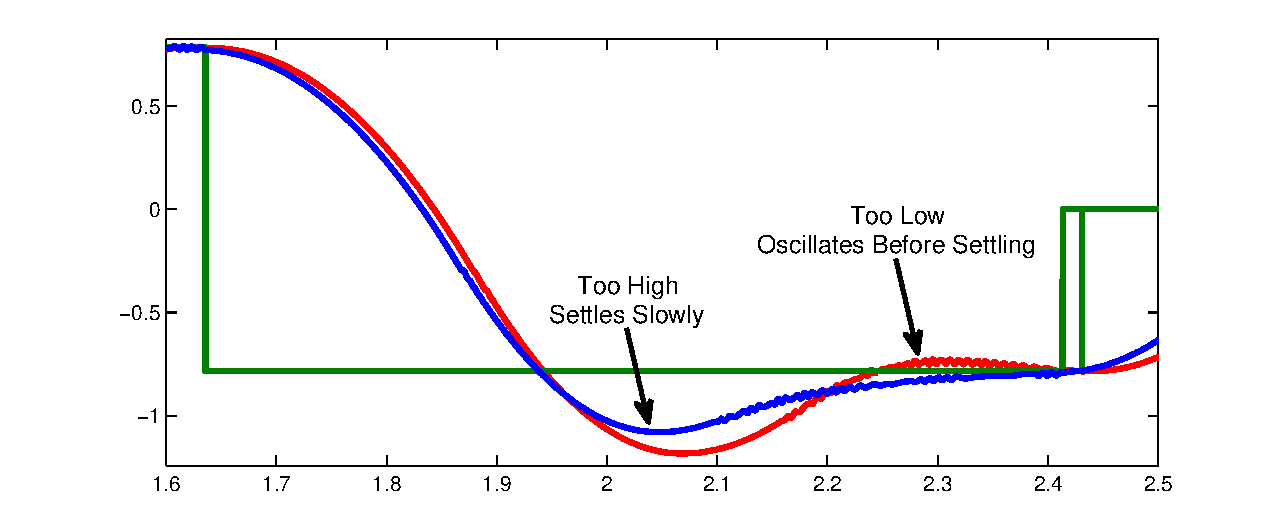
\includegraphics[width=.8\textwidth]{images/ValuesOfKd.pdf}
    \caption{Response For Various Derivative Gains - Incorrect Switching Threshold}
    \label{fig:kd}
\end{figure}

\begin{figure}[htp]
    \centering
    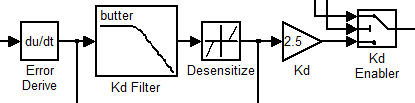
\includegraphics[scale=0.75]{images/Kd.PNG}
    \caption{Simulink Derivative Gain Path}
    \label{fig:simulinkkd}
\end{figure}
